\documentclass[a4paper,11pt]{article}
\usepackage[utf8]{inputenc}

% extra packages
% \usepackage{amsrefs}
% \usepackage[autocite=inline,labelalpha=true]{biblatex}

%\usepackage[top=1in, left=1in, right=1in, bottom=1in]{geometry}
\usepackage{geometry}
\usepackage{amsmath, amssymb}
\usepackage{graphicx}
\usepackage{color}
\usepackage{hyperref}

\newcommand{\ve}{\varepsilon}

%\setlength{\parindent}{0pt}

\begin{document}

\begin{center}
\Large \textbf{Research Statement}

\Large Youngmin Park
\end{center}


\section{Introduction}

My ultimate goal is to understand how modifications to biological neural networks induce normal and pathological brain function. My primary academic interests are to develop dimension-reduction methods for neural network models using dynamical systems theory, and in turn, use these findings to \textit{understand how biological neural networks function and how they are maintained}. Uncovering how individual neurons affect global network behavior is a challenging problem and gives mathematicians ample opportunities to develop theories in this direction.

My research program consists of two sets of complementary questions. The first concerns neural interactions and electrophysiology, which I detail in Section \ref{sec:interactions}. The second concerns neural maintenance and neurophysiology, which I detail in Section \ref{sec:maintenance}.

\section{Neural Interactions}\label{sec:interactions}

The mammalian neocortex is a key region for numerous functions such as sensory perception and integration, generation of fine motor commands, spatial reasoning, and human language \cite{fuster2002frontal}. Over the past century, researchers have established that the neuron is the computational unit of the cortex, and dense networks of neurons ultimately give rise to complex thought. However, the sheer number and density of connections per cubic spatial unit of cortex poses a daunting scientific challenge. Questions about how neurons interact in these networks continue to emerge at a rapid pace. I summarize a few selected questions and my approach to solving them.

\subsection{Previous Work}

\textbf{How does the cortex produce patterned activity?} Spatially-modulated neurons such as head direction, place, and grid cells, produce spatio-temporal brain activity that is fundamental to spatial memory and animal survival. The mechanisms underling this activity are not yet well-understood and are difficult to understand from a mathematical and neurobiological perspective. I introduced a method to reduce the dimension of large neural networks, allowing me to explore the underlying neural mechanisms in great detail. I discovered that interactions between neural adaptation and external inputs contribute to the complex motion of patterned activity in the cortex \cite{park2018scalar}. Only a small set of simple mechanisms can lead to substantial changes in the brain.

\textbf{How does the cortex control brain rhythms?} In addition to spatio-temporal activity, cortical rhythms are ubiquitous and implicated in behavioral tasks such as attention, memory, and motor coordination. Moreover, large cortical networks produce rhythms that are subject to ever-changing concentrations of neuromodulators. The mechanism of how neuromodulators alter rhythms, and therefore attention, is not well-understood. To better understand this mechanism, I introduced a theory to understand acetylcholine's role in changing the synchronization properties of cortical oscillators. My theory showed that neuromodulators alter the phase response curve (PRC) of neurons and therefore alter the large-scale brain rhythms \cite{park2016weakly}. I extended this result to include strongly asynchronous populations of neurons \cite{park2018multiple}, facilitating more realistic studies of small or large networks of heterogeneous neurons.

\textbf{How does the brain process sounds?} The auditory cortex receives signals from the ear drum and cochlea. These auditory signals are processed in simple but important ways. For example, the auditory cortex adapts to constant background noise by responding less over time, but will respond strongly to sudden changes in the auditory environment. This function is critical to the survival of many animals. Numerous optogenetics labs established the differential role of inhibitory neuron subtypes in processing auditory signals. Labs used different paradigms to establish differential effects, so the fundamental role played by each inhibitory subtype was unclear. To better understand the role of neural subtypes, I built a neural model based on the literature capable of reproducing the results of the various paradigms. The model suggests that numerous brain functions can derive from relatively simple circuits, and that the many optogenetic results can be unified under an idealized cortical model \cite{park2020circuit}.

%
%\begin{itemize}
% \item \textbf{Park, Y.} and Geffen, M.N. \textit{A Mechanistic Model of the Auditory Cortex with Inhibitory Subtypes} (in preparation). We introduce a groundbreaking model of cortical responses to complex auditory stimuli, which includes inhibitory subtypes implicated in such auditory processing. The model readily generates hypotheses for the role of these inhibitory subtypes across multiple experimental results.
%
% \item \textbf{Park, Y.}, Shaw, K.M. Chiel, H.J. Thomas, P.J. \textit{The Infinitesimal Phase Response Curve of Oscillators in Piecewise Smooth Dynamical Systems}. European Journal of Applied Mathematics (2018). We provide a first-principles derivation of the phase response curves (PRCs) of oscillators satisfying non-smooth dynamics. This work is a much-needed extension of the half-century-old theory of PRCs.
% 
% \item \textbf{Park, Y.}, Ermentrout, G.B. \textit{Weakly Coupled Oscillators in a Slowly Varying World}. (2016). We extend the theory of weakly coupled oscillators to account for a slowly varying parameter, greatly facilitating more realistic and topical studies using dynamic parameters. 
%  
% \item \textbf{Park, Y.}, Ermentrout, G.B. \textit{Scalar Reduction of a Neural Field Model with Spike Frequency Adaptation}.
% SIAM Journal on Applied Dynamical Systems (2018). We introduce a novel dimension reduction of so-called ``bump'' solutions of non-local neural field models to centroid coordinates. The dimension reduction allows for a comprehensive analysis of the many bifurcations of the system with greater generality than previously possible.
% 
% \item \textbf{Park, Y.}, Ermentrout, G.B. \textit{A Multiple Timescales Approach to Bridging Spiking- and Population-level Dynamics}. (2018). We introduce a powerful theory that robustly accounts for large frequency differences between populations. This substantial contribution enables computational works to operate without the classic restraint of small frequency differences.
% 
% \item \textbf{Park, Y.}, Heitmann, S., Ermentrout, G.B. \textit{The Utility of Phase Models in Studying Neural Synchronization}. Book chapter in Computational Models of Brain and Behavior. Wiley-Blackwell (2017). In this book chapter, we explore how different types of phase response curves and synaptic connections affect the synchronization properties of a network. This chapter is the first to address this relationship directly, and provides a much-needed guideline for future computational studies.
% 
% \item Shaw, K.M., \textbf{Park, Y.}, Chiel, H.J., Thomas, P.J. \textit{Phase Resetting in an Asymptotically Phaseless System}. SIAM Journal on Applied Dynamical Systems (2012). We derive explicit equations for the phase response curve of a planar, piecewise-linear dynamical system. In contrast to existing beliefs, the work proves that transitions between boundaries can have the greatest effect on the phase response curve.
%
%\end{itemize}
\subsection{Ongoing Work}

My theoretical work on neural oscillations falls within the broader work of oscillator theories oriented towards understanding pathological neural behavior such as Parkinsonian tremors, epilepsy, and cardiac alternans. Overall theoretical work in these directions has been promising and tends to use three starting points: mathematically tractable but very abstract models \cite{ott2008low,kopell2014beyond,nicks2018clusters}, particular forms of symmetry \cite{golubitsky1986hopf,golubitsky2003symmetry,murza2011oscillation}, and the \textit{weak coupling} assumption, or more generally, the \textit{linear} approximation \cite{coombes2001phase,ermentrout2002modeling,coombes2012nonsmooth}. The weak coupling assumption has long been an invaluable theoretical tool to understand neural behavior consisting of only small deviations from a known behavior such as quiescence or oscillatory activity. Indeed, the weak coupling assumption has driven much of my work.  %The theories are also intuitively appealing: coupled oscillators interact with each other based on how their synapses filter incoming action potentials.

While these assumptions facilitate theorists to a potent degree and were perhaps close to experimental conditions some decades ago, they are now far from modern experimental conditions. Modern experiments often include \textit{in vivo} conditions, where neurons are often strongly coupled, heterogeneous, and interact nonlinearly. These properties hold in both normal and pathological neural function. It follows that pathologies can not always be understood using abstraction, symmetry, or linearity. Therefore, my field must develop theories that directly address \textit{strongly coupled} networks of \textit{heterogeneous} neurons with \textit{nonlinear} interactions at multiple scales. We must understand the brain as it is.

To this end, \textit{I have formulated a theory of strongly coupled oscillators}. My theory relies on using both a phase angle description and an amplitude description of the oscillator (phase-amplitude coordinates \cite{wilson2019phase,wilson2020phase}). Broadly speaking, I view the phase-amplitude coordinates as coefficients in a Taylor expansion and compute as many coefficients as needed for some desired accuracy. These are called higher-order phase-amplitude coordinates. Using my theory, I am the first to show that strongly coupled oscillators interact based on the cross-correlation of two sets of functions: the higher-order phase-amplitude coordinates and the higher-order derivatives of the oscillator vector fields.

As a first step, I verified my theory using the mathematically tractable complex Ginzburg-Landau (CGL) model. The CGL model is similar to models that classify oscillations in neural models. I diffusively coupled two CGL models with two parameters: $\ve$ for the coupling strength, and $d$ controlling the diffusive coupling complexity. Both parameters significantly affect the phase-locking properties of the coupled CGL models. I show the accuracy of the theory in the left panel of Fig. \ref{fig:cgl}, where the strong coupling theory (green) coincides strongly with the ground-truth (black) relative to the existing coupling theory (red) \cite{wilson2019phase}. 

\begin{figure}[ht!]
	\centering
	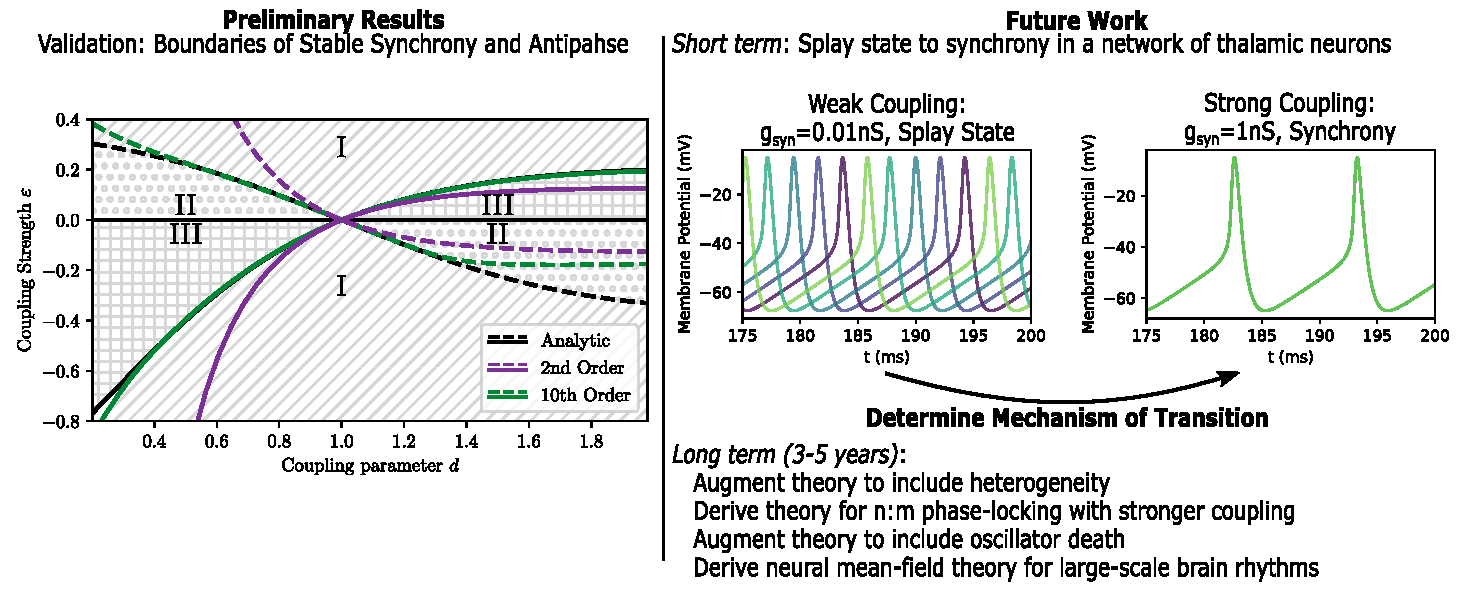
\includegraphics[width=\textwidth]{cgl_twopar_with_future.pdf}
	\caption{Preliminary results and future directions. Left panel: validation of strong coupling theory using diffusively coupled mathematically tractable models. The plot is a two-parameter bifurcation diagram in coupling parameters $\ve$ and $d$. White, gray, and dark gray regions are labeled with synchronous and antiphase oscillations' corresponding stability. Strong coupling theory (green) agrees strongly with ground truth (black) relative to existing theory (red). \textbf{This result shows that my strong coupling theory substantially outperforms existing coupling theory, and is a promising contribution to the vision of multi-level brain theories.} Right panel: An example of future work. With weak coupling, five thalamic oscillators exist in a splay state then transition to synchrony with strong coupling.}\label{fig:cgl}
\end{figure}

I remark that while this result is significant, my theory is not specific to the CGL model and applies to general neural types including non-cortical neurons, and different types of synapses including gap-junction and chemical synapses. My choice of the CGL model with diffusive coupling \textit{is only a first step}. I will build the necessary codebase to implement my strong coupling theory for large, realistic neural networks with this experience.

\subsection{Future Work}

I will further test and apply this theory to neural models with synaptic coupling. For example, I will use my strong coupling theory to determine how varying the synaptic conductance influences transitions from constant and equal phase differences (splay states) to zero phase differences (synchrony).  Figure \ref{fig:cgl} (right panel) shows an example of this phenomenon: five all-to-all synaptically coupled thalamic neurons prefer to spike with equal and constant phase differences when the coupling strength is weak ($g_\text{syn}=0.01$nS) but then transition to synchronous spiking when the coupling strength is relatively large ($g_\text{syn}=1$nS). Strong coupling theory is well-suited to uncover the mechanism of this transition into and out of splay states.

In the long term, I will further develop an understanding of the biological neural networks in several important directions. I will augment my theory to include heterogeneity (including n:m phase-locking), making my theory applicable to far more realistic neural networks. I will augment my theory to include oscillator death to understand interactions between bursting neurons in networks such as subcortical networks and central pattern generators. Finally, I will derive the mean-field equations for neural models (in contrast to existing mean-field theories that use idealized models \cite{ott2008low}) to understand how microscopic neural interactions influence large-scale brain activity. \textit{These essential steps will greatly improve our theoretical understanding of neural oscillations, and in turn, push biological questions in impactful directions.}

\section{Neural Maintenance} \label{sec:maintenance}

While neural interactions are an important part of understanding how brains function, questions of neural maintenance are equally important. Seemingly minor defects at the nanometer-to-micrometer scale can result in serious disorders at the scale of the whole brain. For example, deficits in molecular motor transport in axons are implicated in neurodegenerative diseases such as Pakinson's disease \cite{millecamps2013axonal}. Another example involves pyramidal neurons, the most ubiquitous type of neurons in the mammalian neocortex. They feature tens of thousands of excitatory convergent synaptic inputs, where most incoming synaptic signals terminate on sub-micron bulbs known as dendritic spines \cite{nimchinsky2002structure}. Spines exhibit a significant degree of morphological plasticity \cite{kasai2010structural,holtmaat2009experience} with pathological spine formation implicated in disorders such as Autism spectrum disorder and Alzheimer's disease \cite{penzes2011dendritic}. How spines function and how they are maintained is therefore an important question.

Dendritic spines, as postsynaptic processes, require a high density of surface proteins to function properly. Surface proteins lost through diffusion are replenished by an active process where protein-carrying vesicles squeeze through the neck of the spine and eventually fuse with the spine head \cite{da2015positioning}. The motion of such vesicles has been observed to not involve only translocation, where the motion is unidirectional, but includes corking, where the vesicle gets ``stuck'' in the spine neck, and rejection, where the vesicle initially enters the spine but eventually reverses direction and exits \cite{park2006plasticity,wang2008myosin}. How molecular motors affect changes in direction is the goal of ongoing work.


\subsection{Previous Work}

Observing the movement of vesicles into dendritic spines is challenging due to the lack of high-resolution data. Fine details at the nanometer scale are not possible to resolve in real-time. Therefore, a theoretical approach is a useful tool to understand the possible mechanisms of spine function. Indeed, there is an extensive literature on the effects of molecular motors on cargo dynamics, including the computation of the distribution of cargo velocities \cite{muller2008tug,kunwar2011mechanical}, computing mean first passage times to transport targets on dendritic morphologies \cite{bressloff2009directed,newby2009directed,newby2010random,newby2011asymptotic,bressloff2013metastability}, and the generation of bidirectional motion despite the assumption of symmetry \cite{julicher1995cooperative,guerin2011motion,allard2019bidirectional,portet2019deciphering}. However, these studies often neglect or fix drag forces which could arise from constriction effects in the unique bulbous shape of dendritic spines.

In summary, I converted a mean-field model of constricted vesicle trafficking proposed in \cite{fai2017active} to a fast-slow system, yielding an analytically and numerically tractable version. The model's key parameters include $\phi$, the ratio of (myosin) motors that prefer to push toward the head of the dendritic spine to the motors that prefer to push in the opposite direction, and the effects of confinement $\zeta$, which captures drag forces due to the vesicle moving past a constriction. Through a numerical bifurcation analysis in these parameters, I found that steady-state vesicle velocities appear and disappear through several saddle-node bifurcations. By direct calculations I showed that there can only be unidirectional motion for sufficiently close vesicle-to-spine diameter ratios. This result is consistent with experimental observations of vesicle trajectories in the literature \cite{park2020dynamics}. Vesicles traveling into thin spines with tight constrictions tend to exhibit unidirectional motion, whereas vesicles traveling into wider, stubby spines tend to exhibit bidirectional motion.

While mean-field models are useful with large numbers of agents, sub-micron spines only contain a few dozen myosin motors. The effects of noise are prominent, and we can not rely on mean-field models to fully understand how spines function. Thus I have shifted my attention to understanding how finite numbers of stochastic motors affect the probability of translocation.

\subsection{Ongoing Work}

Before turning to the probability of vesicle translocation, I have decided to focus on the specific question of the mean first passage time (MFPT) to switch velocity. This switching is a well-known ``tug-of-war'' effect \cite{julicher1995cooperative,guerin2011motion} that has not been studied using myosin motors or with constrictions. I have developed an agent-based simulation where individual myosin motors attach and detach with position-dependent rates in order to compute MFPTs. Agent-based simulations motors provide a ground truth to the cargo dynamics, but they are computationally expensive. To obtain mean first passage times (MFPT), roughly 5-10 trials must be run in parallel over 50-100 time units with time steps on the order of 1e-6. My current work involves overcoming the problem of long simulation times through the use of approximations such as the Fokker-Planck equation and the master equation.

The Fokker-Planck equation and corresponding Langevin equation would have been ideal, but they fail to work for our system, which is a class of birth-death models \cite{doering2005extinction}. I have therefore turned to the master equation, which presents its own set of challenges. In existing literature, molecular motors typically do not have spatial dynamics, and have position-independent attachment and detachment rates. A master equation formulation is therefore very straightforward to derive. In contrast, the myosin motor depends on position and velocity, which affect the detachment rates in a way that standard steady-state assumptions are not valid. To account for the dependencies, I included the appropriate position and velocity dependencies into a modified version of the master equation. Some problems remain to be ironed out, but this master equation largely reproduces the MFPT of the agent-based model with a speed improvement in two orders of magnitude.

\subsection{Future Work}

Once all issues have been ironed out, I will turn to the question of how constrictions affect the probability of vesicle translocation and compute the mean first passage time of vesicle translocation. Due to the increasing complexity of the model, I may turn to additional simplifying assumptions and further abstract the model to make this question tractable. The future directions beyond this point are plentiful. For example, protein-carrying vesicles serve as part of a greater maintenance complex that includes maintaining the receptor density, modifying the spine shape and size, and increasing the reliability of postsynaptic spine responses. I will pursue questions on how translocation affects the function of the greater complex, and how the spine maintains an optimal shape for a given function.

Next, spines are distributed throughout a neuron and work together to aid the function of the neuron. In my future research, I will work to understand how the maintenance of individual spines affect the neural response properties. This work will naturally lead to questions of how changes in dendritic spines affect how neurons in small and large networks communicate. This question is vital for understanding the role of defective spines in disorders such as Alzheimer's and autism.


\bibliographystyle{plain}
\bibliography{refs.bib,../youngmin-bard/bio,../youngmin-bard/neuralfield,../youngmin-bard/math,../youngmin-bard/phase,../youngmin-bard/computation,../youngmin-bard/cortex,../thomas-youngmin/notes/spines.bib,../thomas-youngmin/notes/vesicles.bib,../thomas-youngmin/notes/noise.bib,../thomas-youngmin/notes/motors.bib}


\end{document}
